\documentclass{article}
\usepackage{qilin}
\title{ECE159 Exam Review}
\author{QiLin Xue}
\lhead{ECE159}
\rhead{QiLin Xue}
% % \renewcommand{\qedsymbol}{\includegraphics[height=3ex]{kalda.png}}

\newcommand{\equals}{=}

\begin{document}
    \maketitle
    \tableofcontents
    \newpage
    \section{DC Analysis}
    \subsection{Voltage and Current Division}
    For a series circuit, we can calculate the equivalent resistance by adding them.
    \begin{center}
        \begin{tikzpicture}[transform shape, thick]
            \draw (0, 0) to [V, i_>=$i$,
                                l=$V$, invert] (0, 4)
                         to [R, l=$R_1$] (4, 4) node[right] {$A$}
                         to [R, l=$R_2$] (4, 0)
                         to node[ground]{} (0,0); 
            \draw[fill=black] (4,4) circle (1.5pt);
            \draw[fill=black] (4,0) circle (1.5pt);
        \end{tikzpicture}
    \end{center}
    For this circuit, we have:
    \begin{equation}
        R_\text{eq} = R_1 + R_2
    \end{equation}
    and the voltage is given by \textbf{voltage division}:
    \begin{equation}
        V_A = \frac{R_2}{R_1+R_2}V
    \end{equation}
    For a parallel circuit, the effective resistance is the harmonic sum:
    \begin{center}
        \begin{tikzpicture}[transform shape, thick, american currents]
        \draw (0, 0) to [V, i_>=$i$, l=$V$] (0, 4)
                     -- (4,4)
                     to [R,i_>=$i_1$, l=$R_1$] (4, 0)
                     -- (0,0);
        \draw (4,4) -- (8,4)
                    to [R, i_>=$i_2$, l=$R_2$] (8,0)
                    to node[ground]{} (0,0);
        \end{tikzpicture}
    \end{center}
    In this circuit, we have:
    \begin{equation}
        R_\text{eq} = \left(\frac{1}{R_1} + \frac{1}{R_2}\right)^{-1} = \frac{R_1R_2}{R_1+R_2}
    \end{equation}
    and the current in the branches is given by \textbf{current division}:
    \begin{equation}
        i_1 = \frac{R_2}{R_1+R_2}i
    \end{equation}
    \subsection{Mesh and Nodal Analysis}
    In mesh analysis, Kirchoff's Voltage law $\sum V = 0$ is written for each independent loop, and a system of equation is solved. The number of independent loops can be determined by finding the minimum number of wire cuts needed such that there are no loops.

    In nodal analysis, we deal with the potentials at each node and write out Kirchoff's current law $\sum I = 0$ for the current \textit{leaving} (or alternatively, entering) each node for each node where the voltage is unknown.
    \subsection{Superposition}
    Kirchoff's equations are linear. Each term includes only a first power of a current or a voltage, hence we can apply superposition. Let there be $n$ independent voltage sources and $m$ independent current sources. The current in the $j^\text{th}$ wire can be found as:
    \begin{equation}
        I_j = \sum_{k=1}^{n+m} I_j(k)
    \end{equation}
    where $I_j(k)$ is the current in that wire when only the $k^\text{th}$ battery (or current source) is included into the circuit. All other batteries are short circuited and all other current sources are removed by cutting off a connection wire. This same concept can be applied for voltage, but \textit{not} power.
    \subsection{Source Transformation}
    A source transformation is the process of replacing a voltage source $v_s$ in series with a resistor $R$ by a current source $i_s$ in parallel with a resistor $R$, or vice versa. For example, these two circuits are equivalent:
    \begin{center}
        \begin{tikzpicture}[transform shape, thick]
            \draw (3,0) node[right] {$b$} -- (0, 0) to [V,
                                l=$v_s$, invert] (0, 2)
                         to [R, l=$R$] (3, 2) node[right] {$a$}; 
        \end{tikzpicture}
        \begin{tikzpicture}[transform shape, thick, american currents]
            \draw (3,0) node[right] {$b$} -- (0, 0) to [I,
                                l=$i_s$] (0, 2)
                         -- (3, 2) node[right] {$a$}; 
            \draw (1.5,0) to [R, l_=$R$] (1.5, 2);
        \end{tikzpicture}
    \end{center}
    where $v_s=i_sR$.
    \subsection{Thevenin Equivalent Circuit}
    Thevenin's Theorem tells us that any two-terminal circuit can be replaced by an equivalent voltage source $V_\text{th}$ in series with a resistor $R_\text{th}$. These are related via:
    \begin{equation}
        \label{thevenin}
        R_\text{th} = \frac{V_\text{th}}{I_\text{sc}}
    \end{equation} 
    To calculate $V_\text{th}$, we find the \textit{open circuit} voltage between the two terminals. To calculate $R_\text{th}$, there are three options:
    \begin{enumerate}
        \item Remove all independent voltage and current sources and calculate the equivalent resistance across the terminals.
        \item Connect the two terminals via a wire with negligible resistance. Calculate the current $I_\text{sc}$ through this wire and we can calculate $R_\text{th}$ using equation \ref{thevenin}.
        \item Inject a test current $I_\text{test}$ from one node, and measure the potential difference $V_\text{test}$. The resistance is then:
        \begin{equation}
            R_\text{th} = \frac{V_\text{test}}{I_\text{test}}
        \end{equation}
    \end{enumerate}
    \subsection{Norton Equivalent Circuit}
    Similar to Thevenin, we can also perform a source transformation such that we can replace any subcircuit element with an independent current source connected to a resistor in parallel. Note that calculating the equivalent resistance is done in the same way.
    \section{Operational Amplifiers}
An operational amplifier (op amp) is an active circuit element designed to perform mathematical operations of addition, subtraction, multiplication, division, differentiation, and integration.
\begin{center}
    \begin{circuitikz}[line width=1pt]
        \draw
        (0,0) node[op amp,yscale=1](opamp){} 
        (opamp.+) to[short, -o] ++(-.5,0) node[left]{$v_2$}
        (opamp.-) to[short, -o] ++ (-.5,0) node[left]{$v_1$}
        (opamp.out) to[short, -o] ++ (.5,0) node[right]{$v_0$}
        ;
    \end{circuitikz}
    
\end{center}
It is equivalent to the following circuit:
\begin{center}
    \begin{tikzpicture}[transform shape, thick]
        \draw  (-2,2) to [short, -o] (-2,2) node[left] {$v_1$} -- (0, 2) to [R, l=$R_i$, v_<=$v_d$] (0,-2) to [short, -o] (-2,-2) node[left] {$v_2$};

        \draw (6,0) node[right] {$v_0$} to [short, -o] (6,0) to [R, l=$R_0$] (3,0) to [V, l_=$A(v_2-v_1)$] (3, -1.5) node[ground]{};
    \end{tikzpicture}
\end{center}
where $A \gg 1$ is known as the open-loop voltage gain. The input resistance $R_i$ is typically very big.
\subsection{Ideal OP Amp}
For an ideal OP Amp, we have an infinite open-loop gain, infinite input resistance, and zero output resistance. This gives the following results:
\begin{itemize}
    \item The currents into both input terminals are zero.
    \item Voltage across input terminals are zero.
\end{itemize}

\newpage
\subsection{Types of Amplifiers}
Here is a list of common amplifiers:
\begin{itemize}
    \item Inverting Amplifier:
    \begin{equation}
        v_0 = -\frac{R_2}{R_1} v_i
    \end{equation}
    \begin{center}
        \begin{tikzpicture}[transform shape, thick]
            \draw (0,3) node[left] {$v_i$} to [short, -o] (0,3) to [R, l=$R_1$] (3,3);

            \draw
            (5,2.5) node[op amp,yscale=1](opamp){} 
            (opamp.+) to ++ (-0.5,0) to ++ (0, -2) node[ground]{}
            (opamp.-) -- (3,3)
            (opamp.out) to[short, -o] ++ (1,0) node[right] {$v_0$};
            
            \draw (3,3) -- (3,4) to [R, l=$R_2$] (6.5,4) -- (6.5,2.5);
        \end{tikzpicture}
    \end{center}
    \item Noninverting amplifier:
    \begin{equation}
        v_0 = \left(1+\frac{R_2}{R_1}\right)v_i
    \end{equation}
    \begin{center}
        \begin{tikzpicture}[transform shape, thick]
            \draw (0,3) node[ground] {} to [R, l=$R_1$] (3,3);

            \draw
            (5,2.5) node[op amp,yscale=1](opamp){} 
            (opamp.+) to[short,-o] ++ (-0.5,0) node[left] {$v_i$}
            (opamp.-) -- (3,3)
            (opamp.out) to[short, -o] ++ (1,0) node[right] {$v_0$};
            
            \draw (3,3) -- (3,4) to [R, l=$R_2$] (6.5,4) -- (6.5,2.5);
        \end{tikzpicture}
    \end{center}
    \item Voltage follower:
    \begin{equation}
        v_0 = v_i
    \end{equation}
    \begin{center}
        \begin{tikzpicture}[transform shape, thick]

            \draw
            (5,2.5) node[op amp,yscale=1](opamp){} 
            (opamp.+) to[short,-o] ++ (-0.5,0) node[left] {$v_i$}
            (opamp.-) -- (3,3)
            (opamp.out) to[short, -o] ++ (1,0) node[right] {$v_0$};
            
            \draw (3,3) -- (3,4) -- (6.5,4) -- (6.5,2.5);
        \end{tikzpicture}
    \end{center}
    \item Summer:
    \begin{equation}
        v_0 = -\left(\frac{R_f}{R_i}v_1 + \frac{R_f}{R_2}v_2 + \frac{R_f}{R_3}v_3\right)
    \end{equation}
    \begin{center}
        \begin{tikzpicture}[transform shape, thick]
            \draw (0,3) node[left] {$v_2$} to[short, -o] (0,3) to [R, l=$R_2$] (2,3) -- (3,3);
            \draw (0,4) node[left] {$v_1$} to[short, -o] (0,4) to [R, l=$R_1$] (2,4) -- (2,3);
            \draw (0,2) node[left] {$v_3$} to[short, -o] (0,2) to [R, l=$R_3$] (2,2) -- (2,3);

            \draw
            (5,2.5) node[op amp,yscale=1](opamp){} 
            (opamp.+) to ++ (-0.5,0) to ++ (0, -2) node[ground]{}
            (opamp.-) -- (3,3)
            (opamp.out) to[short, -o] ++ (1,0) node[right] {$v_0$};
            
            \draw (3,3) -- (3,4) to [R, l=$R_f$] (6.5,4) -- (6.5,2.5);
        \end{tikzpicture}
    \end{center}
    \item Difference Amplifier:
    \begin{equation}
        v_0 = \frac{R_2}{R_1}(v_2-v_1)
    \end{equation}
    \begin{center}
        \begin{tikzpicture}[transform shape, thick]
            % \draw (0,3) node[left] {$v_2$} to[short, -o] (0,3) to [R, l=$R_2$] (2,3) -- (3,3);
            % \draw (0,4) node[left] {$v_1$} to[short, -o] (0,4) to [R, l=$R_1$] (2,4) -- (2,3);
            % \draw (0,2) node[left] {$v_3$} to[short, -o] (0,2) to [R, l=$R_3$] (2,2) -- (2,3);

            \draw
            (5,2.5) node[op amp,yscale=1](opamp){} 
            (opamp.+) to ++ (-0.5,0) to ++ (0, -1) to [R, l=$R_2$] (6.5, 1) node[ground] {}
            (opamp.-) to ++ (-0.5,0) to ++ (0,1) to [R, l=$R_2$] (6.5,4) -- (6.5,2.5)
            (opamp.out) to[short, -o] ++ (1,0) node[right] {$v_0$};
            
            \draw (0,4) node[left] {$v_1$} to [short, -o] (0,4) to [R, l=$R_1$] (3.29,4);
            \draw (0,1) node[left] {$v_2$} to [short, -o] (0,1) to [R, l=$R_1$] (3.29,1);

        \end{tikzpicture}
    \end{center}
\end{itemize}
\section{First Order Circuits}
\subsection{Overview of Capacitors and Inductors}
A capacitor is able to store charge such that the voltage across it is:
\begin{equation}
    V = \frac{q}{C}
\end{equation}
where $C$ is the capacitance. Differentiating both sides, we have:
\begin{equation}
    \frac{dV}{dt} = \frac{i}{C} \implies i = C\frac{dV}{dt}
\end{equation}
Since the current cannot be infinite, the voltage across a capacitor must be differentiable (i.e. smooth). When multiple capacitors are in series, the equivalent capacitance is:
\begin{equation}
    C_\text{eq} = \left(\frac{1}{C_1}+\frac{1}{C_2} + \cdots\right)^{-1}
\end{equation}
For multiple capacitors in parallel, the equivalent capacitance is:
\begin{equation}
    C_\text{eq} = C_1+C_2+\cdots
\end{equation}
The energy stored in a capacitor is given by:
\begin{equation}
    U = \frac{q^2}{2C} = \frac{1}{2}CV^2 = \frac{q}{2V}
\end{equation}
An inductor maintains a voltage that resists a change in current (i.e. via Lenz's Law). This means the voltage across a resistor is:
\begin{equation}
    V = -L\frac{di}{dt}
\end{equation}
where $L$ is the inductance. Since the voltage across cannot be infinite, the current across it has to be differentiable. When inductors are added in series, the equivalent inductance is:
\begin{equation}
    L_\text{eq} = L_1 + L_2 + \cdots
\end{equation}
and in parallel:
\begin{equation}
    L_\text{eq} = \left(\frac{1}{L_1} + \frac{1}{L_2}+\cdots\right)^{-1}
\end{equation}
The energy stored in an inductor is:
\begin{equation}
    U = \frac{1}{2}Li^2
\end{equation}
\begin{idea}
    For $RL$ and $RC$ circuits, at time scales much shorter than the characteristic times $\tau = RC$ or $\tau = L/R$ (i.e. right after a switch is opened), the capacitor's charge and inductor's current remain almost constant. In particular, if a capacitor was chargeless, its voltage remains almost zero (i.e. short circuit). If there was no current in an inductor, its current remains zero (i.e. inductor may be considered to be broken). If a capacitor had a charge $Q$ corresponding to a voltage $V_0$, its voltage remains essentially constant (i.e. it acts and can be substituted by a battery of voltage $V$). Similarly, if an inductor had a current $I_0$, it can be substituted by a respective constant current source. If we try to forcefully break the current through an inductor by switching it off, a rapid fall of current $I$ creates a huge voltage $-L\frac{dI}{dt}$ which usually leads to a spark at the switch.
    \vspace{2mm}

    At time scales much larger than the characteristic times, the situation is reversed: the inductor can be considered a short-circuiting wire, and capacitor as an insulator. This is because all the currents and voltages tend exponentially towards the equilibrium state so that the different from the equilibrium value $\Delta \propto e^{-t/\tau}$: the capacitor charge is almost constant, hence there is no current, and the inductor current is almost constant, hence no voltage.
\end{idea}
\subsection{Natural Response}
Since resistors provide a ``decaying response'' (see the mechanical analogy section), it is expected that RC and RL circuits have a decaying exponential, when there are no voltage sources:
\begin{equation}
    x(t) = x(0)e^{-t/\tau}
\end{equation}
where $x(0)$ is the initial value of a quantity (current or voltage), and $\tau$ is the time constant. For RC circuits, we have $\tau = RC$ and for RL circuits, we have $\tau = L/R$. It is the characteristic time for which a certain quantity decreases by a factor of $\frac{1}{e}$. For an $RC$ circuit, we can derive this from the equation:
\begin{equation}
    i_c + i_r = 0 \implies C\frac{dV}{dt} + \frac{V}{r} = 0
\end{equation}
though I prefer working with Kirchoff's Voltage Law:
\begin{equation}
    -\frac{dq}{dt}R - \frac{q}{C} = 0
\end{equation}
This is because we see a similar structure for the inductor:
\begin{equation}
    -iR - L\frac{di}{dt} = 0
\end{equation}
Notice the connection between $q$, $i$, and $\frac{di}{dt}$. This is important when formulating the mathematics behind complex AC circuits later.
\subsection{Step Responses}
When we have a sudden change (i.e. a voltage or current source is added), the circuit may behave slightly differently. Since it is a first order circuit, we should still expect an exponential pattern. If we add a constant voltage or current term to the differential equation above, we can easily solve for it. Alternatively, we can abuse the fact that it is a linear differential equation so we can write the general solution as:
\begin{equation}
    \text{complete response} = \text{natural response} + \text{forced response} 
\end{equation}
or
\begin{equation}
    v = v_n + v_f
\end{equation}
or:
\begin{equation}
    v = v_t + v_{ss}
\end{equation}
Here, $v_t$ is the transient response, and it will die out with time. The steady state response $v_{ss}$ is the behaviour of the circuit a long time after an external excitation is applied. As a result, we can write out the voltage of a capacitor:
\begin{equation}
    \boxed{v(t) = v(\infty) + [v(0)-v(\infty)]e^{-t/\tau}}
\end{equation}
Taking the derivative and rearranging:
\begin{equation}
    i_c(t) = \frac{V_\text{th}-V(t_0)}{R_\text{th}} e^{-t/\tau}
\end{equation}
and similarly for an RL circuit:
\begin{equation}
    \boxed{i(t) = i(\infty) + [i(0) -i(\infty)]e^{-t/\tau}}
\end{equation}
\section{AC Circuits}
In AC circuits, we may have combinations of inductors, capacitors, resistors, and sinusoidal voltage sources. We are concerned only with the steady state response. We can do this with phasors. Suppose the voltage frequency is $\omega$, then the \textbf{impedances} are:
\begin{align}
    Z_R &= R \\ 
    Z_C &= \frac{-j}{\omega C} = \frac{1}{j\omega C} \\ 
    Z_L &= j\omega L
\end{align}
where $j^2=-1$ is the imaginary number. The \textbf{admittance} is the inverse of the impedance. Using these impedances, we can effectively ``solve'' an AC circuit in the same way that we solve a DC circuit.
\subsection{Interpreting Complex Numbers}
Note that we can convert between cartesian and polar forms of complex numbers via:
\begin{equation}
    a + jb = r \angle \theta
\end{equation}
where $r = \sqrt{a^2+b^2}$ and $\tan\theta = \frac{b}{a}$. Suppose that the voltage is in the form of:
\begin{equation}
    V = V_0 \angle \theta
\end{equation}
This simply means that the voltage is a sinusoidal wave with a magnitude of $V_0$, and has a phase shift of $\theta$, where the phase shift is calculated relative to some reference (usually the input voltage). We can interpret complex current in the same way.
\subsection{Resonance and Filters}
Resonance occurs when:
\begin{equation}
    \omega_c = \frac{1}{\sqrt{LC}}
\end{equation}
A filter is a circuit that is designed to pass signals with desired frequencies and reject or attenuate others. A \textbf{passive filter} consists of only passive elements $R$, $L$, and $C$. There are four different types of filters:
\begin{itemize}
    \item Low-pass: passes low frequencies and stops high frequencies (i.e. RC)
    \item High-pass: passes high frequencies and stops low frequencies (i.e. CR)
    \item Band-Pass: Passes frequencies within a frequency band. (i.e. LCR)
    \item Band-stop: Passes frequencies outside a frequency band. (i.e. RCL)
\end{itemize}
The transfer function is defined as
\begin{equation}
    H(\omega) = \frac{V_o}{V_i}
\end{equation}
describes the increase/decrease in voltage at a given load. The transfer function for each filter at key frequencies are given below:
\begin{center}
    \begin{tabular}{|c|c|c|c|}
        \hline
        Type      & $H(0)$ & $H(\infty)$ & $H(\omega_c)$        \\ \hline
        Low Pass  & $1$    & $0$         & $\frac{1}{\sqrt{2}}$ \\ \hline
        High Pass & $0$    & $1$         & $\frac{1}{\sqrt{2}}$ \\ \hline
        Band Pass & 0      & 0           & 1                    \\ \hline
        Band Stop & 1      & 1           & 0                    \\ \hline
        \end{tabular}
\end{center}
\subsubsection{Magnitude Scaling}
In decibel scale, we define:
\begin{equation}
    H_\text{dB} = 20\log_{10}H
\end{equation}
\subsection{Power}
\textbf{Notation:} I will use bolded variables to represent complex numbers: The most general power is the \textbf{complex power:}
\begin{align}
    \bm{S} &= P + jQ \\
    &= \bm{V}_\text{rms}\left(\bm{I}_\text{rms}\right)^* \\ 
    &= V_\text{rms}I_\text{rms} \angle (\theta_v-\theta_i) \\ 
    &= \frac{1}{2}\bm{V_m}\bm{I_m}^* \\ 
    &= \bm{Z}I_\text{rms}^2
\end{align}
We will define $\theta=\theta_v-\theta_i$. Here, $P$ is the \textbf{real power}:
\begin{equation}
    P = S\cos(\theta_v-\theta_i)
\end{equation}
and $S=\sqrt{P^2+Q^2}$ is the \textbf{apparent power}. The \textbf{reactive power} is:
\begin{equation}
    Q = S\sin(\theta_v-\theta_i)
\end{equation}
\subsubsection{Optimal Power}
The optimal resistance and reactance of a load such that the maximum power is delivered to it in an AC circuit is given when:
\begin{align}
    R_L &= \sqrt{R_\text{th}^2 + (X_\text{th}+X_\text{L})^2} \\ 
    X_\text{L} &= - X_\text{th}
\end{align}
If both these criteria are satisfied, then:
\begin{equation}
    P_\text{max} = \frac{|\bm{V}_\text{th}|^2}{8R_\text{eq}}
\end{equation}
In general, the average power delivered to the load is
\begin{equation}
    P = \frac{1}{2}|\bm{I}|^2 R_L = \frac{|\bm{V}_\text{th}|^2R_L/2}{(R_\text{th}+R_L)^2+(X_\text{Th}+X_L)^2}
\end{equation}
\begin{warning}
    Do not confuse this with the power delivered to a load in a DC circuit:
    \begin{equation}
        P = \frac{V_\text{th}^2}{4R_\text{th}}
    \end{equation}
    the reason for the extra factor of $\frac{1}{2}$ in the AC circuit case, is that the power is a sinusoidal wave and we are looking for only the \textit{average power}.
\end{warning}
\subsubsection{Power Factor}
We can define the power factor to be:
\begin{equation}
    \text{pf} = \cos\theta = \cos(\theta_v - \theta_i)
\end{equation}
such that:
\begin{equation}
    P = S \cdot \text{bf}
\end{equation}
However, note that for each power factor, there are two possible values of $\theta$ that satisfy it. As a result, we define:
\begin{itemize}
    \item \textbf{Leading pf:} $\theta<0$
    \item \textbf{Lagging pf:} $\theta>0$
\end{itemize}
Special cases:
\begin{itemize}
    \item Resistor: $pf=1$
    \item Inductor: $pf = 0$ lag
    \item Capacitor $pf = 0$ lead
    \item RL: $0<pf<1$ lag
    \item RC: $0<pf<1$ lead
    \item RLC: $0<pf<1$ lag or lead. Specifically, it depends on the sign of:
    \begin{equation}
        \omega L - \frac{1}{\omega C}
    \end{equation}
\end{itemize}
\subsubsection{Power Factor Correction}
The process of increasing the power factor without altering the voltage or current to the original load is known as power factor correction. It can be viewed as the addition of a reactive element (usually a capacitor) in parallel with an inductive load in order to make the power factor closer to unity.

An inductive load is modeled as a series combination of an inductor and a resistor.

The value of the required shunt capacitance $C$ is determine to be:
\begin{equation}
    C = \frac{P(\tan\theta_1-\tan\theta_2)}{\omega V_\text{rms}^2}
\end{equation}
where $\theta_1$ is the initial power factor angle and $\theta_2$ is the final angle. This equation is derived from the following principles.
\begin{itemize}
    \item We want the real power $P$ to be constant.
    \item We want to change the power factor, which depends solely on the power factor angle. As a result, we can only change the imaginary part $Q$.
    \item To do so, we need to figure out how much of the imaginary power do we want to increase/decrease, and then perform phasor math (and using impedances) to figure out the capacitance $C$ necessary to do so. Specifically, if we need to increase the reactance by $Q_C$ to achieve the desired $\text{pf}$, we select the capacitance:
    \begin{equation}
        X_c = \frac{V_\text{rms}^2}{Q_c} \quad \text{ or } \quad C = - \frac{Q_c}{\omega V_\text{rms}^2}
    \end{equation}
\end{itemize}
We can draw a power triangle to illustrate this:
\begin{center}
    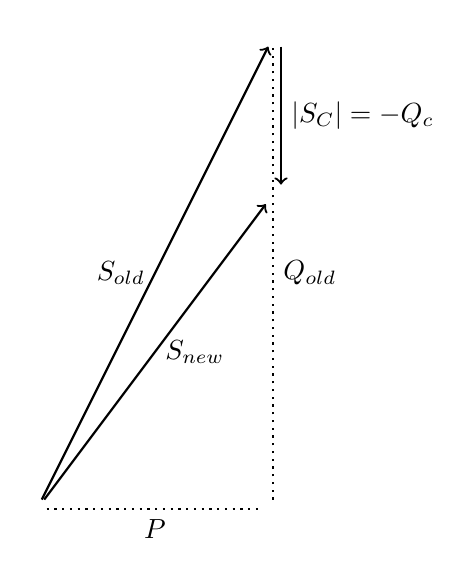
\begin{tikzpicture}
        \node (O) at (0,0) {};
        \node (A) at (3,0) {};
        \node (B') at (3,4){}; 
        \node (B) at (3,6) {};
        \node (B2') at (3.1,4){}; 
        \node (B2) at (3.1,6) {};
    
        \draw[thick, ->] (O) -- (B) node[midway,left] {$\bm{S}_\text{old}$};
        \draw[thick, ->] (O) -- (B') node[midway,right] {$\bm{S}_\text{new}$};
        \draw[thick, ->] (B2) -- (B2') node[midway,right] {$|\bm{S}_\text{C}|=-Q_c$};

        \draw[thick, dotted] (O) -- (A) node[midway,below] {$P$};
        \draw[thick, dotted] (A) -- (B) node[midway,right] {$Q_\text{old}$};
    \end{tikzpicture}
\end{center}
From this, note that:
\begin{equation}
    \bm{S}_\text{old} + \bm{S}_C = \bm{S}_\text{new}
\end{equation}
so we can define (note that we defined $Q_C$ is a negative quantity here):
\begin{equation}
    Q_\text{new} = Q_\text{old} + Q_c
\end{equation}
which gives:
\begin{equation}
    \frac{Q}{P} = \tan \theta_\text{old}
\end{equation}
and:
\begin{equation}
    \frac{Q_\text{new}}{P} = \tan \theta_\text{new}
\end{equation}
To make the power factor unity, we set $Q_C = -Q_L$ where $Q_L$ is the reactance of the load.
\subsubsection{Apparent and Effective Value}
The effective value of a periodic current is the DC current that delivers the same average power to a resistor as the periodic current:
\begin{equation}
    I_\text{eff} = \sqrt{\frac{1}{T}\int_0^T i^2 \dd{t}}
\end{equation}
for an arbitrary periodic function $x(t)$, the effective (or \textbf{root mean square} value) is:
\begin{equation}
    X_\text{rms} = \sqrt{\frac{1}{T}\int_0^T x^2 \dd{t}}
\end{equation}
We can convert between the rms value and the peak values of a sinusoidal function:
\begin{equation}
    V_\text{rms} = \frac{V_m}{\sqrt{2}},\quad I_\text{rms} = \frac{I_m}{\sqrt{2}}
\end{equation}
\subsubsection{Random Things when Doing Practice}
\begin{itemize}
    \item $|\bm{S}|$ and $|\bm{Z}|$ are scalar multiples of each other. As a result, $\bm{S}$ has the same power factor angle as $\bm{Z}$: $\bm{S}=\bm{Z}I_\text{rms}^2$.
    \item The angular frequency is not the same as frequency:
    \begin{equation}
        \omega = 2\pi f
    \end{equation}
\end{itemize}
This conversion factor also works if we are working with complex voltages.
% \subsubsection{Average and Instantaneous Power}
% The instantaneous power is the power at any instant of time:
% \begin{equation}
%     p(t) = i(t)v(t)
% \end{equation}
% The average power is the average of the instantaneous power over one period:
% \begin{equation}
%     P = \frac{1}{T} \int_0^T p(t) \dd{t}
% \end{equation}
% or:
% \begin{equation}
%     P = \frac{1}{2}V_mI_m \cos(\theta_V-\theta_I)
% \end{equation}
% where $\theta_V-\theta_I$ is the different in phase between voltage and current.
% \begin{idea}
%     A resistive load ($R$) abosrbs power at all times, while a reactive load ($L$ or $C$) absorbs zero average power.
% \end{idea}
% \subsubsection{Maximum Average Power Transfer}
% \begin{theorem}
%     The maximum average power transfer, the load impedance $Z_L$ must be equal to the complex conjugate of the Thevenin impedance $Z_\text{Th}$:
%     \begin{equation}
%         Z_L = Z_\text{th}^*
%     \end{equation}
%     and when this occurs, we say that the load is matched to the source.
% \end{theorem}
% From this, we can derive that the maximum average power transfer is
% \begin{equation}
%     P_\text{max} = \frac{|V_\text{th}|^2}{8R_\text{th}}
% \end{equation}
% \subsubsection{Apparent Power and Power Factor}
% The \textbf{apparent power} $S$ is the product of the RMS values of voltage and current:
% \begin{equation}
%     S = V_\text{rms}I_\text{rms}
% \end{equation}
% The power factor is a dimensionless ratio that gives the ratio of average power to apparent power:
% \begin{equation}
%     \text{pf} = \frac{P}{S} = \cos(\theta_v - \theta_i)
% \end{equation}
% where $\theta_v-\theta_i$ is the \textbf{power factor angle}.
% \subsubsection{Complex Power}
% The complex power is given in the form of:
% \begin{equation}
%     S = P + jQ = V_\text{rms}I_\text{rms} \angle (\theta_v-\theta_i)
% \end{equation}
% where $P = \Re(S) = S\cos(\theta_v-\theta_i)$ is the real power and $Q=\Im(S)=S\sin(\theta_v-\theta_i)$ is the reactive power. The complex power contains \textit{all} relevant power information in a given load.
% \subsubsection{Conservation of AC Power}
% \begin{theorem}
%     The average power is conserved in AC circuits. In fact, all forms of AC power are conserved: Instantaneous, real, reactive, and complex.
% \end{theorem}
\end{document}

